\documentclass[12pt,a4paper]{article}
\synctex=1
\usepackage[utf8]{inputenc}
\usepackage[margin=1cm]{geometry}
\usepackage{graphicx}
%\usepackage{verbatim}
\usepackage{listings}
\usepackage{textcomp}
\usepackage{courier}
\usepackage{libertine}
\usepackage{pgfornament}
\usepackage{eso-pic}
\usepackage[hangul]{kotex}
\linespread{1.3}

\title{
	\centering
	\pgfornament[width=12cm,color=teal]{84}\\
	\vspace{1cm}
	\fontsize{50}{50} \selectfont {컴퓨터 그래픽스 입문}\\
		\pgfornament[width=12cm,color=teal]{88}\\
	\vfill}
\author{
	\LARGE
	\begin{tabular}{rl}
		\hline
		학번 : & 2016110056\\ 
		학과 : & 불교학부 \\
		이름 : & 박승원\\
		날짜 : & \today\\
		\hline
	\end{tabular}\vspace{2cm}
	\\

\includegraphics[width=0.5\textwidth]{logo.jpg}
	}
\date{}


\begin{document}
\maketitle
\pagenumbering{gobble}
\noindent
\lstset{language=C++, columns=flexible, tabsize=4, frame=shadowbox, showstringspaces=false, breaklines=true, upquote=true, basicstyle=\normalsize}
\newpage
\section*{Lab 11. Texturing}
	
\begin{verbatim}
Pick a relatively low resolution 3D model from the thingiverse.

Step 1. Apply the butterfly subdivision. Show the difference before and after applying it. (3pt)

Step 2. Apply the Loop subdivision. Show the difference before and after applying it. (3pt)

Step 3. Show the difference between the butterfly and the Loop subdivision. (4pt)
\end{verbatim}

블렌더의 대표 마스코트인 몽키를 triangle subdivision했다.
위가 loop이고, 아래가 butterfly이다.
그런데, normal에서의 버그가 있어서인지, 트라이앵글을 나누어서 노말을 자체적으로 계산했을때,
원숭이의 얼굴 반만이 나왔다.

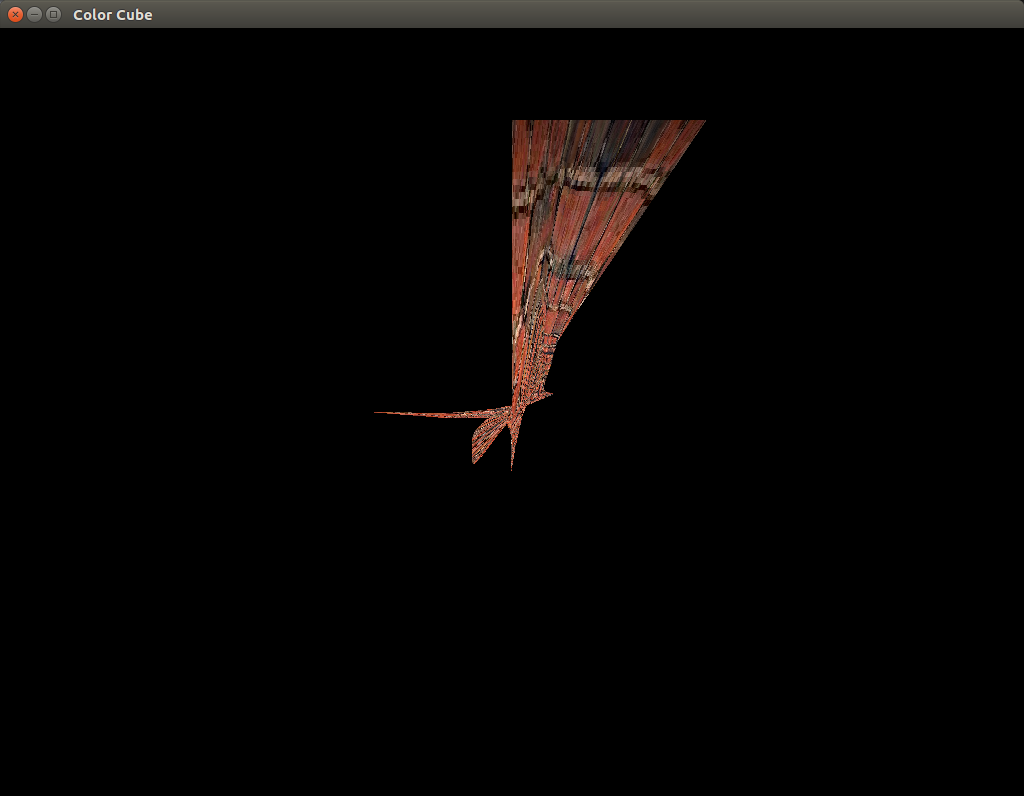
\includegraphics[width=\textwidth]{1.png}

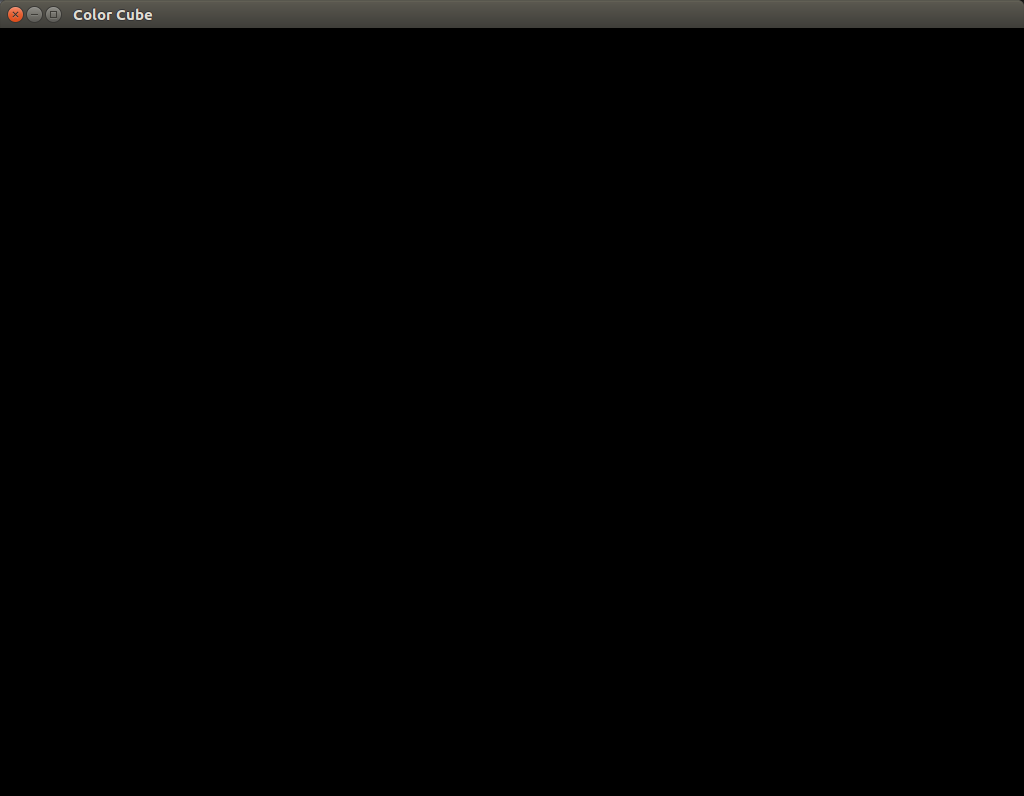
\includegraphics[width=\textwidth]{2.png}
\lstinputlisting[]{src/globject.cc}
\lstinputlisting[caption=main함수]{src/val2.cpp}

\end{document}
